\chapter{Superexchange Interaction}
Ultracold atoms in optical lattices enables a wide variety of Hamiltonians to be mapped to the system. Thus, quantum simulations of various models can be conducted, as the interactions within the system can be tuned through manipulation of external fields. An example of this is the spin-spin interactions between particles described by the Ising and Heisenberg model \cite{Bloch2012}. One such action is the spin-exchange interactions, which is an effective interaction that does not any direct coupling between spins. The spin-exchange interaction is observed for electrons as the interplay between the Coulomb force and exchange symmetries. This interaction is short ranged, as it is governed by the overlap of wavefunctions. However, at longer distances  the \textit{superexchange} interaction can be observed, where the interaction is mediated through higher-order exchanges \cite{Anderson1959}.

\section{Theoretical Model}
The simplest setting for examining the superexchange interaction is a double well system occupied by a pair of bosons of different spin states, which are denoted by $\ket{\uparrow}$ and $\ket{\downarrow}$.\\
As the system consists of bosons in a lattice, the Hamiltonian is simply a variant of the Bose-Hubbard Hamiltonian, which takes the different spins into account
\begin{equation}
	\hat{H} = \sum_{\sigma = \uparrow , \downarrow} \left[ -J \left( \hat{a}_{\sigma \mathrm{L}}^{\dag} \hat{a}_{\sigma \mathrm{R}} + \hat{a}_{\sigma \mathrm{R}}^{\dag} \hat{a}_{\sigma \mathrm{L}} \right) - \frac{\Delta}{2} \left( \hat{n}_{\sigma \mathrm{L}} - \hat{n}_{\sigma \mathrm{R}} \right)   \right] + U \left( \hat{n}_{\uparrow \mathrm{L}} \hat{n}_{\downarrow \mathrm{L}} + \hat{n}_{\uparrow \mathrm{R}} \hat{n}_{\downarrow \mathrm{R}} \right) \; . \label{eq:SpinHubbard}
\end{equation}
Here, L and R denote the left and right well respectively, $J$ is the tunnel matrix element, $U = U_{\uparrow \downarrow}$ is the on-site interaction between two atoms of opposite spin, and $\Delta$ is a potential bias \cite{Trotzky2008}. Like in the regular Bose-Hubbard model, the matrix elements can be calculated through the overlap of wavefunctions. Specifically in the case of well localized atoms is the use of a Wannier basis favourable, whereby the matrix elements are given by 
\begin{equation}
	U = U_{\uparrow \downarrow} = g \times \int \mathrm{d}^3 x \; |w_{\mathrm{L},\mathrm{R}} (\boldsymbol{x})|^4 \; ,
\end{equation} 
where $g = \frac{4 \pi \hbar^2 a}{m}$, and $a$ and $m$ are the scattering length and the mass of the atoms. Furthermore,
\begin{equation}
	J = J_{\uparrow} = J_{\downarrow} = - \int \mathrm{d}x \ w_{R}^*(x) \left( - \frac{\hbar^2}{2 m} \nabla ^2 + V(x) \right) w_{L}(x) \; ,
\end{equation}
where $V(x)$ is the confining potential, and $w_{\mathrm{L},\mathrm{R}} (\boldsymbol{x})$ is a Wannier function localized at either the left or right well \cite{Kuklov2003}.\\
Equation \eqref{eq:SpinHubbard} provides a general description of spinful bosons in a double well. However, in the limit of dominating interactions $U \gg J$, the probability of doubly occupation of a well is highly suppressed. Hence, upon starting in the subspace of singly occupied wells spanned by $\ket{\uparrow,\downarrow}$ and $\ket{\downarrow,\uparrow}$, the states $\ket{\uparrow \downarrow, 0}$ and $\ket{0, \uparrow \downarrow}$ can only be reached as virtual intermediate states through second order tunneling processes.
\begin{figure}[h]
	\centering
	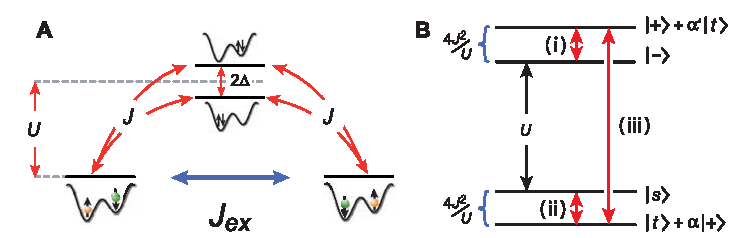
\includegraphics[width=0.9\textwidth]{Figures/SXEschematic.pdf}
	\caption{\textit{Schematics of superexchange interaction. (\textbf{A}) Second order hopping between states $\ket{\uparrow,\downarrow}$ and $\ket{\downarrow,\uparrow}$ is achieved through virtual, intermediate states. (\textbf{B}) Energy levels for $\Delta = 0$ and $U \gg J$. Process (ii) depicts the superexchange exchange interaction, while (i) is the coupling of doubly occupied states through correlated tunneling of atom pairs. Both doublets are coupled by a first order tunneling process (iii), which is highly suppressed in the Mott regime. Figure adopted from \cite{Trotzky2008}.}}
	\label{fig:superexchange}
\end{figure}
This is an example of a superexchange interaction coupling the states $\ket{\uparrow,\downarrow}$ and $\ket{\downarrow,\uparrow}$. This is visualised in figure \ref{fig:superexchange}.A, where the coupling of the two singly occupied states is achieved through the energetically higher-lying, doubly occupied states. Thus, the upper states are virtual, as they are merely an intermediate step in the coupling.
Assuming zero potential bias ($\Delta = 0$), the effective coupling strength between $\ket{\uparrow,\downarrow}$ and $\ket{\downarrow,\uparrow}$ is given by $J_{\mathrm{ex}} = 2 \frac{J^2}{U}$, which can be derived through second order perturbation theory.\\
Consider the case of $U \gg J$. Since the tunnelling matrix element is so small, the kinetic part of the Hamiltonian \eqref{eq:SpinHubbard} can be considered a perturbation. Due to the high value of $U$, employing a basis of single occupied states, $\rho = \{ \ket{\uparrow , \downarrow} , \ket{ \downarrow, \uparrow} , \ket{\uparrow,\uparrow} , \ket{\downarrow,\downarrow} \}$, is favourable. At first order, applying $\hat{H}_J$ to any member of $\rho$ will yield a state outside the basis. Thus, all first order contributions vanish. To second order, the perturbation is given by
\begin{align}
	H_{a,b}^{\mathrm{eff}} = \sum_{a \neq b} \frac{ |\bra{a} \hat{H}_{J}\ket{b}|^2}{\varepsilon_a - \varepsilon_b} \; , \label{eq:2ndorderpertubation}
\end{align}
where $\varepsilon$ denotes the energy of the respective state. For the same reasons as for the first order, no contributions come from $a,b \in \rho$. Therefore, one must consider all possible doubly occupied states. Thus, including the operator $\mathds{1} - \hat{P}_{\rho}$, which projects out of the subspace $\rho$, one can write equation \eqref{eq:2ndorderpertubation} as
\begin{align}
	H_{a,b}^{\mathrm{eff}} &=  - \braket{a|\hat{H}_J \frac{\mathds{1} - \hat{P}_{\rho}}{\hat{H}_U} \hat{H}_J|b} \nonumber \\
	&= \sum_{n \notin \rho} \braket{a|\hat{H}_J|n} \left( \braket{n |\hat{H}_U | n} \right)^{-1} \braket{n|\hat{H}_J|b} \; .
\end{align}
For $J_{\sigma} = J $ and $U_{\uparrow\uparrow} = U_{\downarrow\downarrow} = U_{\uparrow\downarrow}/2$, one can write the effective Hamiltonian in the basis $\rho$ as
\begin{align}
\hat{H}_{\mathrm{eff}} = -J_{\mathrm{ex}} \begin{pmatrix}
           1 & 1 & 0 & 0 \\
           1 & 1 & 0 & 0 \\
           0 & 0 & 1 & 0 \\
           0 & 0 & 0 & 1 
         \end{pmatrix} \; , \label{eq:BosonHamilEff}
\end{align}
where $J_{\mathrm{ex}} = 2 \frac{J^2}{U}$ \cite{Duan2003}. Diagonalizing this Hamiltonian yields eigenstates in the form of a spin triplet, $\ket{t}$ with energy $E_t = -2 J_{\mathrm{ex}}$, and a spin singlet, $\ket{s}$ with energy $E_s = 0$. This is illustrated in the bottom part of figure \ref{fig:superexchange}.B. The upper doublet displayed in figure \ref{fig:superexchange}.B contains further eigenstates of the Hamiltonian \eqref{eq:SpinHubbard} with doubly occupation. However, deep within the Mott regime ($U \gg J$) the doubly occupied states only exists as virtual states. Furthermore, the coupling between the two doublets is through a first order tunneling process, which is highly suppressed in the Mott regime. Thereby the coupling between the two doublets can be neglected, and one only has to consider the lower doublet, whose effective Hamiltonian is that of equation \eqref{eq:BosonHamilEff}, where the coupling is mediated through the superexchange interaction.\\
Utilizing the eigenspectrum of the effective Hamiltonian (eq. \eqref{eq:BosonHamilEff}) one can express the Hamiltonian through the projection operator into the triplet subspace, $\hat{P}_t$, such that
\begin{equation}
	\hat{H}_{\mathrm{eff}} = -2 J_{\mathrm{ex}} \hat{P}_t \; . 
\end{equation}  
The triplet projection operator has the important property that it can be described by spin operators, $\hat{P}_t = \frac{3}{4} \hat{\boldsymbol{S}}_{\mathrm{L}} \cdot \hat{\boldsymbol{S}}_{\mathrm{R}}$, where $\hat{\boldsymbol{S}}_{\mathrm{L,R}}$ are the spin operators for the left and right site respectively. By discarding the constant term, the Hamiltonian \eqref{eq:BosonHamilEff} can be mapped to that of an isotropic Heisenberg model, yielding \cite{Trotzky2008}
\begin{align}
	\hat{H}_{\mathrm{eff}} &= -2 J_{\mathrm{ex}} \hat{\boldsymbol{S}}_{\mathrm{L}} \cdot \hat{\boldsymbol{S}}_{\mathrm{R}} \nonumber \\
	&= - J_{\mathrm{ex}} \left( \hat{S}_{\mathrm{L}}^{+} \hat{S}_{\mathrm{R}}^{-} + \hat{S}_{\mathrm{L}}^{-} \hat{S}_{\mathrm{R}}^{+} \right) - 2 J_{\mathrm{ex}} \hat{S}_{\mathrm{L}}^{z} \hat{S}_{\mathrm{R}}^{z} \; , \label{eq:twositeFerro}
\end{align}
where 
\begin{align*}
\hat{\boldsymbol{S}}_{\mathrm{L,R}} &= \left(  \hat{S}_{\mathrm{L,R}}^{x} , \hat{S}_{\mathrm{L,R}}^{y} , \hat{S}_{\mathrm{L,R}}^{z} \right)^{T} \\
\hat{S}_{\mathrm{L},\mathrm{R}}^{+} &= \left( \ket{\uparrow}\bra{\downarrow} \right)_{\mathrm{L},\mathrm{R}} \\
\hat{S}_{\mathrm{L},\mathrm{R}}^{-} &= \left( \ket{\downarrow}\bra{\uparrow} \right)_{\mathrm{L},\mathrm{R}} \\
\hat{S}_{\mathrm{L},\mathrm{R}}^{z} &= \left( \hat{n}_{\uparrow \; \mathrm{L},\mathrm{R}} - \hat{n}_{\downarrow \; \mathrm{L},\mathrm{R}} \right)/2 \\
\hat{S}_{\mathrm{L},\mathrm{R}}^{\pm} &= \hat{S}_{\mathrm{L},\mathrm{R}}^{x} \pm i \hat{S}_{\mathrm{L},\mathrm{R}}^{y}
\end{align*}
Thus, the superexchange interaction of bosons is ferromagnetic, which accounts for the ground state being the spin triplet configuration.

Applying a potential bias $\Delta > 0$ lifts the degeneracy of the two intermediate states, thus modifying the effective coupling. For $J,\Delta \ll U$ the coupling becomes
\begin{equation}
	J_{\mathrm{ex}} = \frac{J^2}{U + \Delta} + \frac{J^2}{U - \Delta} \; . \label{eq:Jex_delta}
\end{equation}
Hence, by tuning the bias to $\Delta > U$ one can change the sign of the coupling, thereby switching between ferromagnetic and antiferromagnetic superexchange interactions \cite{Trotzky2008}.\\
If the vibrational level splitting in each potential well is much larger than all relevant energy scales, the two-site model can be extended to an entire one-dimensional lattice \cite{Trotzky2008}. Thus, within the Mott-Insulator regime ($U \gg J$) with unity filling, the full system can be treated as an isotropic Heisenberg spin chain
\begin{equation}
	\hat{H} = - J_{\mathrm{ex}} \sum_{\left\langle j, k \right\rangle} \left( \hat{S}_{j}^{+} \hat{S}_{k}^{-} + \hat{S}_{j}^{-} \hat{S}_{k}^{+} \right) - 2 J_{\mathrm{ex}} \sum_{\left\langle j, k \right\rangle} \hat{S}_{j}^{z} \hat{S}_{k}^{z} \; , \label{eq:HeisenbergChain}
\end{equation}
where $\left\langle j, k \right\rangle$ denotes summing over neighbouring sites. In the process of deriving equation \eqref{eq:twositeFerro} and \eqref{eq:HeisenbergChain} a constant energy shifts was left out, however, this can be compensated for by applying an external magnetic field.\\
When describing information transfer through a spin chain, one is most often describing the propagation of a single spin impurity. In this case the first term in equation \ref{eq:HeisenbergChain}, which describes the longitudinal spin coupling, is merely an energy offset, which can be neglected \cite{Fukuhara2013}.  